
\chapter{Failure Diagnosis for Industrial Automation Plant}
\label{chap:problem_description}

This chapter uses an example of industrial automation plant to present the
problem of fault diagnosis. After a short description of the technological
process it shows two cases of failures. Then the types of failures are
discussed, and what approaches are adopted in industrial and academic
practices.

\section{Case Study of the Automated System}

An instance of the real automated systems is exploited to explain the problem of
failure diagnosis. It is a dust cleaner at an aluminium smelter. The Figure
\ref{fig:pi_diagram} depicts a simplified Piping and Instrumentation (P\&I) of
the system.

\subsection{Technological process}

\begin{figure}
  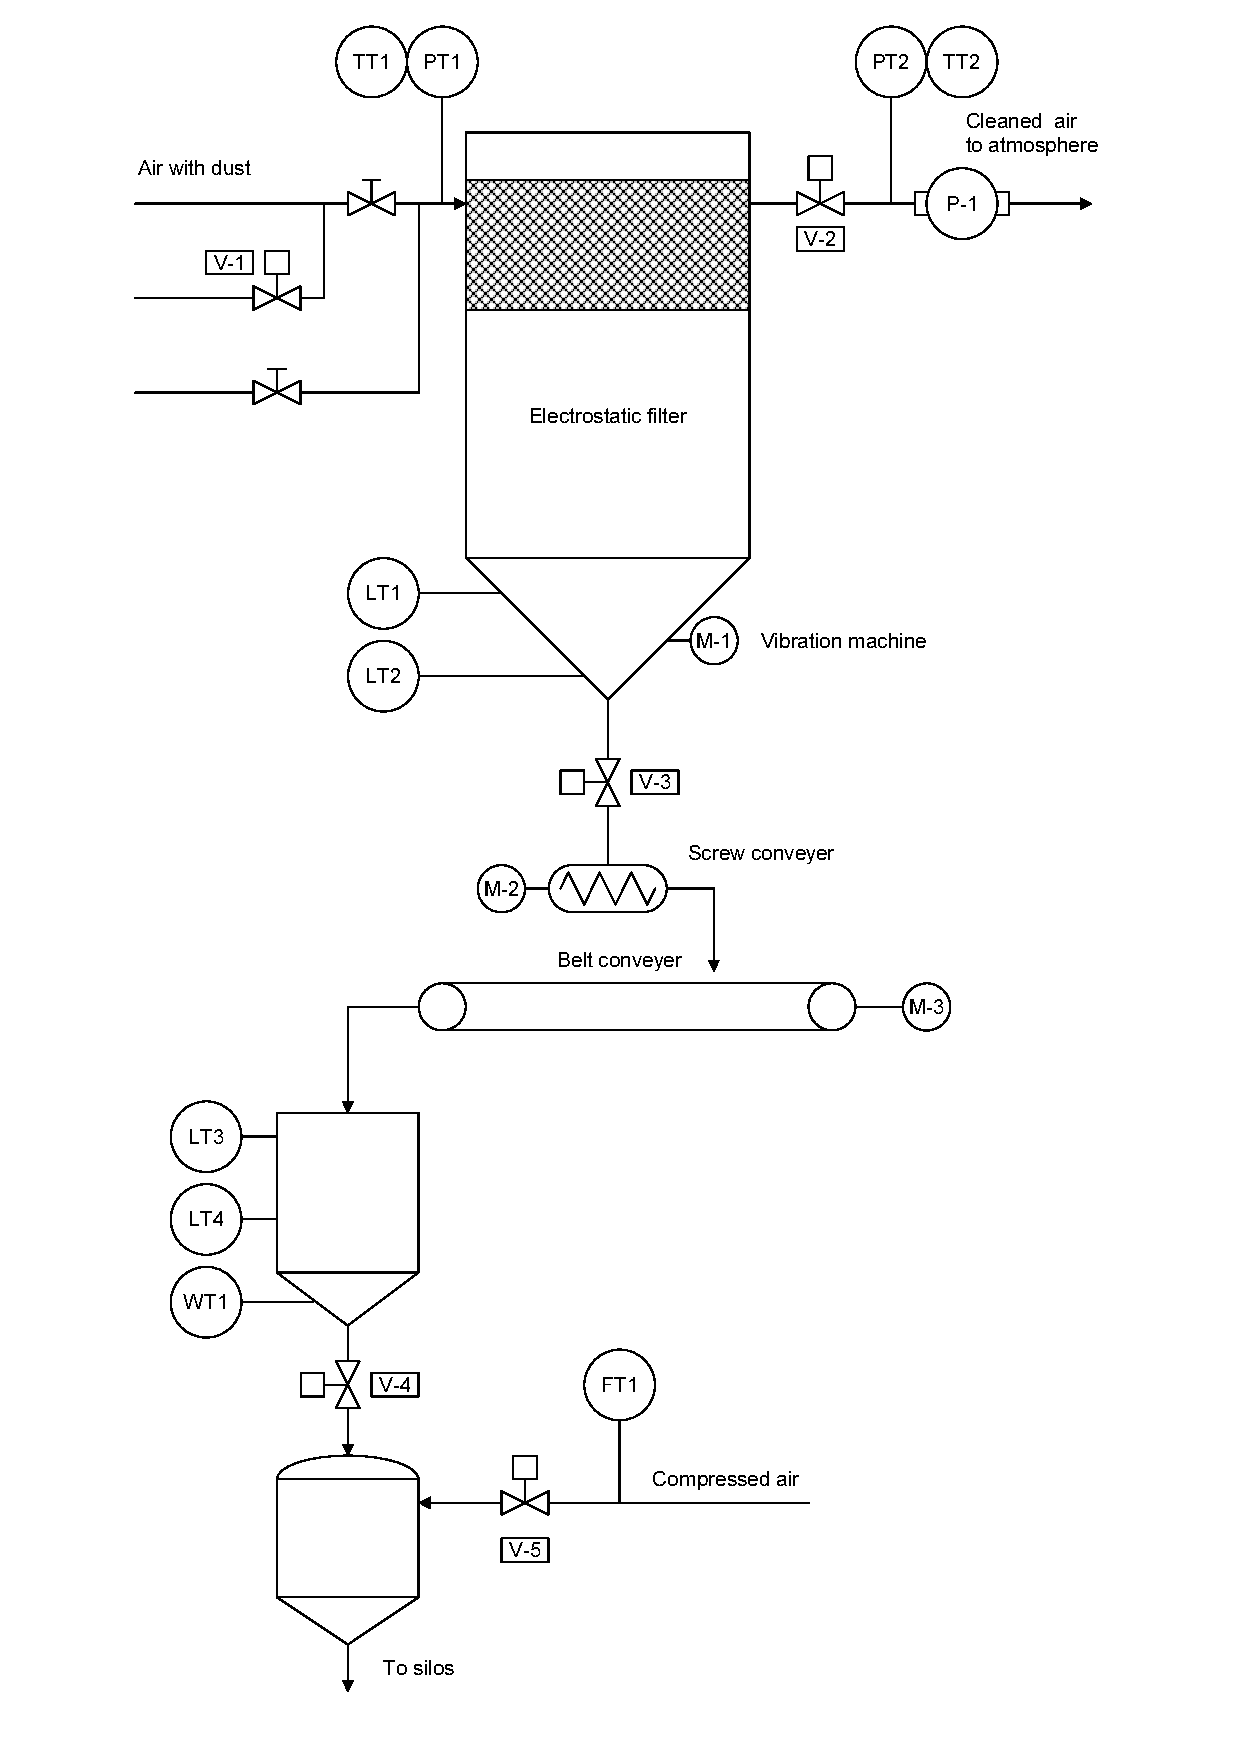
\includegraphics[width=\textwidth, keepaspectratio, angle=0] 
  {process-and-instrument-drawing.pdf}
  \caption{Piping and Instrumentation (P\&I) diagram of a dust cleaning system
  at an aluminium smelter}
  \label{fig:pi_diagram}
\end{figure}

For the given system two flows can be distinguished in the technological
process.
The first is the air flow which is blown trough a series of containers (the
figure depicts only one container, for simplicity). Each container is equipped with an
electrostatic filter.
The second flow is the flow of a dust. The dust comes with the air, sticks to
the filter, and then falls down to the bunker. Periodically the dust collected
in the bunker is transported out to a silos.

For the proper dust cleaning, the following parameters of the air flow have to
be maintained: a constant difference between the output and the input
pressures of the container, and a temperature at the input of the container. The
pressure is regulated by the valve $V$--2, which changes the area flow before
the pump $P$--1.
The temperature is regulated by the valve $V$--1 which changes the area flow 
of a preheated air. The air at the entrance of the filter is, thus, a mix of
the the polluted air and the preheated air. The temperature of this mix should
be higher then a certain point such that no condensation inside of the container
is guaranteed.

When the amount of the dust collected at the bottom of the container reaches a
necessary volume, i.e. it reaches a certain level, the dust is removed by the
screw conveyer. The gate valve $V$--3 is normally opened, since the screw of the
conveyer blocks the flow of the dust automatically when it is stopped. The belt
conveyer, in its turn, starts to work whenever one of the screw conveyers
starts. It delivers the dust to a dust bucket.

The dust bucket collects the dust until a volume of the dust is enough to pass
it down, to a pneumatic container. Then the gate valve $V$--4 opens and the
dust fills the container. Then the gate valve $V$--4 closes and the gate valve
$V$--5 opens allowing the compressed air to come to the container. Under a high
pressure the mix of the dust and the air is transported to a silos.

Periodically, in order to prevent sticking of the dust to the walls of the
container with electrostatic filters, the vibration machine $M$--1 has to be
switch on for a few seconds.


\subsection{Control System}

% Description of the control system (Siemens, etc.) (picture of PLC, Control
% station and etc, showing distributed nature of the system)

The control system consists of a PLC (Siemens Simatic S7--300
\cite{simatic_s7_300}), remote acquisition modules and an operator station
(with Siemens WinCC software) connected via industrial network. The PLC is
mounted near the field equipment, the operator station is located a few hundreds
meters away. 

The control systems has a few control cycles. Starting to the bottom-up
direction, the first cycle controls emptiness of the dust bucket with two level
sensors, $LT3$ and $LT4$. When a level of the dust reaches the high level
sensor $LT3$, the system starts to empty the bucket with the pneumatic container
until a level of the dust reaches the low level sensor $LT4$. The weight meter
$WT1$ is used to collect the statistic, and its measurements can be also used to
evaluate the amount of the dust in the container. The air flow meter $FT1$ is
aimed to collect statistical data too.

The second control cycle regulates the filling of the dust bucket. When the
dust level in the bucket is lower then the high level sensor $LT3$, and there is
an enabling signal from the upper (with respect to the material flow) control
cycle, it turns on the belt conveyer and enables a signal to one of the upper
control cycles (each container with its filter has its own control cycle).
Either the level of the dust in the bucket reaches the high level sensor $LT3$
or there is no any enabling signals from the upper control cycles, then the belt
conveyer stops.

The third control cycle regulates the level of the dust in the container
with the filter (the cycle is the same for each container). When the dust level
reaches the high level sensor $LT1$, it gives enabling signal to the below
control cycle of the belt conveyer and waits for enabling signal from it. After
receiving the enabling signal, the control cycle switches on the screw conveyer.
Ether the container becomes empty, i.e. the dust level decreases below the low
level sensor $LT2$, or the control cycle receives disabling signal from the
below control cycle, then it switches the screw conveyer off.

The forth control cycle regulates an order the containers with the filters
should be emptied. If more than one container is ready, i.e. the level of the
dust reached its high level sensor, then the first container has a priority,
since the speed it is filled with dust is faster. Then the second
container is emptied and so forth.

The fifth control cycle switches on vibration machines periodically, but only
when the container is being emptied.

All the actuators of the system can be in three states: disabled for operation,
manual control or automatic control. A signal corresponding to
the current state of each actuator is received by the PLC.


\subsection{Failures of the system}

The system can be affected by different types of failures, which may be
classified into the following categories with respect to likelihood the failure
occurs (the first type has the highers rate of occurrence):

\begin{itemize}
  \item Failures of the technological process
  \item Failures of mechanical devices
  \item Failures of electric and electronic components of the control system
\end{itemize}

Moreover, the failures can be external or internal with respect to the given
system. Yet another type of failure is one when malfunction of the system's
behavior is caused by an inconsistent human (operator) intrusion; it has left
outside of the scope. Some of the possible failures are described further,
according to the above classification.

\subsubsection{Failures of the technological process}

The technological failures might be caused by deviation of properties of the
materials involved in the process. Particularly in this system, a deviation of
the dust's or air's humidity can result in that the dust sticks to the filter,
to the walls of the container and to pipes, and obstructs the flow of the material.
Whereas the temperature of the air (low value of which is the main reason for
the condensation) is controlled, the humidity is not measured.

The air, coming to the pneumatic container has neither a temperature nor
humidity control. Additionally, the rise of the material humidity may happen due
to a leak of rainwater from the building's roof, and etc.

In general, technological failures are hard to predict, since there is
usually a little of statistical information for the particular process, if any. 

\subsubsection{Failures of the mechanical devices}

Malfunction of field mechanical devices, probably, is the most frequent reason
the automatic systems fail. Firstly, the field devices are exposed to hard
environmental conditions, such as temperature, vibration, humidity,
electromagnetic field, mechanical impact and etc. Secondly, they are normally
complex devices, composed of many other components, and thus the failure rate of
a complex device is higher then the highest failure rate of its modules.
A common solution adopted in industry is that all the actions performed under
each individual device, conditions under with the equipment is used, a time
duration it works, and etc. are journalized. These statistical information is
later used to plan and perform the maintaining and repairing.

The above presented system has following devices with mechanical parts and
parts which can be affected mechanically (e.g. by the flow of a material):
\begin{itemize}
  \item Butterfly valves $V$--1, $V$--2 and gate valves $V$--3, $V$--4, $V$--5.
  The weakest part of a valve is its actuator, which contains a plenty of
  moving components. Beside this, the valve's core is subject to abrasion. 
  \item The screw conveyer and the belt conveyer. These devices have a lot of
  moving components either, where the belt as the weakest part.  
  \item Electric motors $M$--1 -- 3 and pump $P$--1, which
  are subject to mechanical and electric damages.
  \item Weight meter $WT1$, with its fore tension meters which are subject to
  degradation.
  \item Fork level meters $LT1$ -- $4$. The forks are subject to abrasion.
  \item Pressure meters $PT1$, $PT2$. The drive mechanism of a pressure meter is
  the subject to stacking, dirt and oil clogging. 
\end{itemize}

All the above potential mechanical failures, the most of the listed above devices
contain electronic and electric components, which can have their one failures. 

\subsubsection{Failures of electric and electronic components}

Due to enormous amount electric and especially electronic components used in
modern manufacturing industry, it is quite impossible to make a classification
of all the failures which might occur, and it is seems useless to have such
information at the level of industrial automation, since a fault of a single
component most likely results in the failure of entire device it contains.
Instead, complex characteristics are used in order to be able to estimate 
possible faults. One of the well know parameters is the Mean time between
failures (MTBF). Another, relatively modern standard IEC 61511 also defines a
set of characteristics (MTBF and IEC 61511 are described briefly later).

\subsection{Examples of the systems' failures}

This work does not consider the question of faults prevention. The fact of a
fault occurrence has to be assumed, since the problem of the failure is not
only that it may lead the necessity to interrupt the technological process,
delay for delivery of spare parts and row materials. The major problem is that
one failure can sequentially cause other failures which may spread further
and so forth, with exponential growth, provoking a catastrophic impact at the
end.

As an example, the system presented in this chapter was subjected to 
some failures observed by the author of this work. These failures are
interesting from the point of view of their propagation.

In the first case the high level sensor $LT3$ failed while the system was at the
state of refilling the dust bucket. Since one of the conditions the control
system has to stops the filling is that the dust bucket is full, it was
delivering more and more material. The material overflowed the bucket in great
quantity, causing clogging of ventilation holes of the control system (which
later resulted in some spare parts change), and blocking entrance to the
building. The failure was spotted occasionally; elimination of its consequences
took a few days. It was discovered later, that the failure of the fork level
sensor was caused by blocking it with a wet material that, in its turn was
caused by a high humidity in the building. Thus, the technological failure has
propagated to a failure of sensor, and later to a failure of electronic
components.

Another example is related not to a failure of particular equipment, but to the
control system. In this case the shaft of the motor $M$--2 was left not
connected to the screw conveyer after a maintenance service. Thus, when the
motor is switched on, the screw conveyer does not rotates and blocks the flow of
material. When the system started to empty the first container, i.e.
the control cycle responsible for unload of the container with electrostatic
filter had enabling signal to the below control cycle, and the control cycle
responsible for the filling of the dust bucket, in its turn, had an enabling
signal for the upper control cycle, the system was found infinitely trying to
fill the dust bucket from the first container. If not spotted, this failure
could lead to the overfilling of the container, clogging of the filters and air
channels, and pollution of the environment.

These illustrative examples of failures are showing importance of the failures
detection. If a particular single fault can not be detected, at least one
the propagating effects should be observed. The earlier a failure is detected
the less damaging impact it leads to. The evidence of this fact can be stressed
by a numerous examples and case studies: \cite{james_failure},
\cite{forensic_failre_analysis}, \cite{arora_failures_2007} to mention a few.


\section{Industrial and Academical Analytical Approaches}
% Overview of Failure Detection and Diagnostic Approaches

% From an industrial perspective, to-do list for failures:  
%  . Prevent
%  . Detect. 
%  		. What is necessary to detect, and what is not? FMEA
%  		. Is it possible to detect? Formal methods. 
%  . Diagnose
%  		. Formal methods
%  . Reconfigure the system (fault tolerance)
%  		. Formal methods


\subsection{Prevent, Detect, Isolate and Recover}

From the point of view of an automation engineer a failure is an event which has
to be, firstly, \emph{prevented}, then \emph{detected} and \emph{diagnosed}.
It is clear that nobody can guarantee that a failure can not occur under all
circumstances. As it was shown by examples in the previous section, failures
also tend to propagate, causing other failures with a greater impact.
Thus, a general assumption is that the failures are not avoidable, but the
failure propagation may be prevented.

Determinization of all the potential failures is a separate difficult task.
This problem is addressed with the different qualitative and quantitative 
analytical methods at the design stage while the development of a new system.

The next step, after all the possible system's failures are found and
evaluated, is to decide if each failure can be detected. The problem is that the
effects of a failure may be difficult to observe. There can be a lack of
the technological process parameters deviation, lack of equipment (sensors) or
time (performance). Even if observed, the failure may be not easy to distinguish
from a normal system's behaviour. Moreover, it might happen that the
observed effects caused by one failure can not be distinguished (or, in other
words, isolated) from effects caused by another failure. These two failures may
required different reactions, thus they has to be distinguished. The problem of
failure detection and isolation is know as a diagnosability problem.

After a failure is detected and analysed, the system usually is desired to
continue operating properly, possibly at a reduced level of performance, but not
to fail completely. Such property of systems is called \emph{fault tolerance}.
In industrial applications the property of fault tolerance is usually achieved
by redundancy, i.e. is by duplication of critical components or functions of a
system. The major form of redundancy in manufacturing are:
\begin{itemize}
  \item Hardware redundancy, such as double module redundancy or triple module
  redundancy
  \item Information redundancy, such as error detection and correction methods. 
  \item Functional redundancy, when the same input produces an equivalent
  output through different media or different principles
\end{itemize}

For example, in the dust cleaning systems, presented in this work, the three
containers with electrostatic filters may be considered as a form of hardware
redundancy. A level of dust in the dust bucket can be measured by mean of its
weight and by the fork level sensors, thus, providing a form of information
redundancy. When the system works in the non-automatic mode, based on decisions
of its operator, actuation of motors can be performed both via the
software control system and locally by hardware buttons - functional
redundancy. 

The problem of fault-tolerance is out the scope of this work. We proceed with a
brief description of some qualitative and quantitative analytical approaches
adopted in industry, such as Failure Mode and Effects Analysis (FMEA), Mean time
between failures (MTBF), reliability online databases and IEC 61511
standard. Then a Simulation approach is described as a way for failure
validation, and, finally, the formal methods approach. Some of these approaches
can be considered as pure industrial ones, while other widely used in both
industrial and academic fields. The formal methods is seen as a pure academic
response to the problem of failures diagnosis.


\subsection{Failure Mode and Effects Analysis}
% http://medqi.bsd.uchicago.edu/documents/FailureModesandEffectsAnalysis_FMEA_1.pdf
% https://static.squarespace.com/static/515082bbe4b0910b244269db/t/516d6e4ce4b0f84b6313c3ed/1366126156359/FMEA%20Webinar%20core%20tools.pdf

FMEA is an exhaustive analysis of systems, an analytical tool to identify,
quantify, prioritize and evaluate the risk of possible failures in order to
reduce risk of failures, ensure that failures are detectable and prevent failure
from happening. Assuming that any failure which was determined can occur, it
is necessary to figure out what negative impact of each failure (of type of
failures) can be, i.e. what failures must to be detected, what are wished to
be detected, and what are not, since the failure detection may be an expensive
process in terms of time, increasing complexity and costs of the whole system.

FMEA is described in the {IEC 60812} standard, and consists of:
\begin{itemize}
  \item System analysis - how interactions among systems may fail
  \item Design analysis - how product design may fail
  \item Process analysis - how processes that make the product might fail
  \item Design analysis -  focuses on how machinery that perform processes might fail
\end{itemize}
 
A chart with steps which are necessary to perform according to FMEA methodology
is depicted in Figure \ref{fig:fmea_chart}.

\begin{figure}[th]
  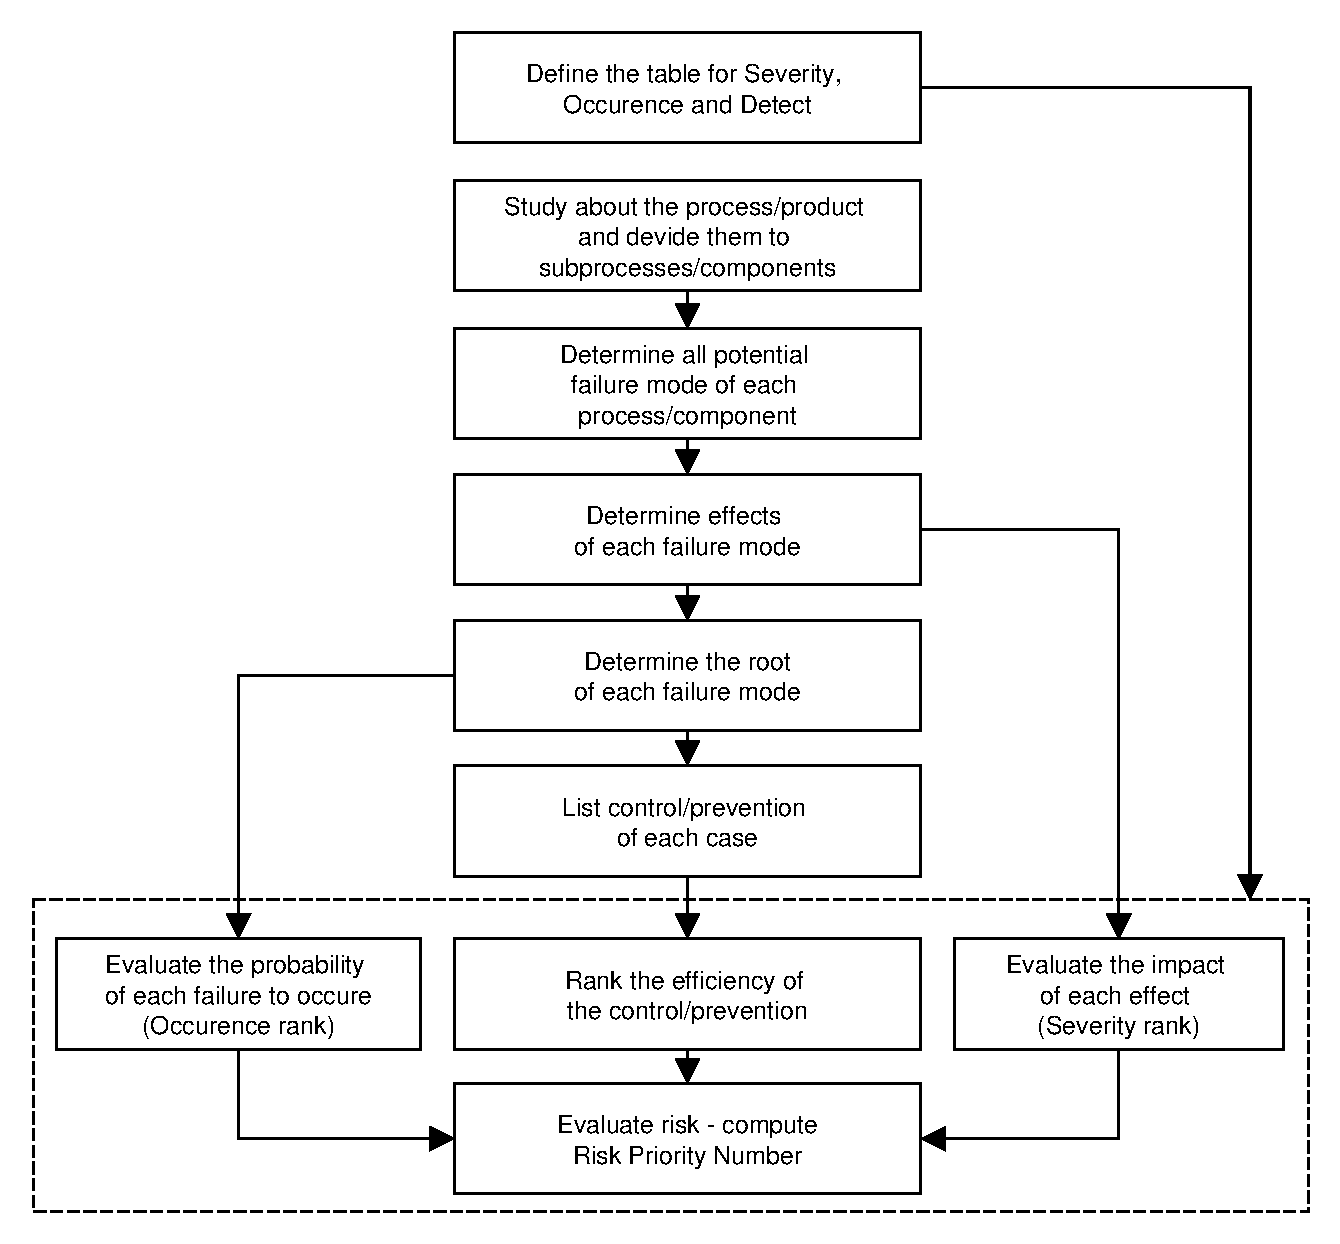
\includegraphics[width=\textwidth, keepaspectratio, angle=0]
  {fmea_chart.pdf}
  \caption{The necessary steps for FMEA methodology}
  \label{fig:fmea_chart}
\end{figure}

FEMA involves reviewing as many components, assemblies, and subsystems as
possible to identify failure modes, and their causes and effects. It also
involves a lot of human resources: experts and practitioners in particular
industrial fields \cite{tague_quality_2010}.
That is why this tool is considered as a relatively expensive approach, and is
adapted mostly for life-critical systems, related to military area, automotive,
gas and oil industry, health-care and life-support activity. There are other,
less costly but yet similar knowledge based analytical approaches, presented in
literature, for instance the adapted for industrial use Process Mapping
\cite{what_is_a_process_map}, and State analyses \cite{ruiz_state_2000}.


\subsection{Mean Time Between Failures} 

Mean time between failures (MTBF) is a statistical mean value for error-free
operation (between two failures) of an electronic device during the normal working life. The MTBF does not apply
to an individual component, it always refers to the phase with constant failure
rate (i.e. without early or wear failures). The higher the MTBF, the less often
the component fails and the more reliable it is. In addition to the MTBF value, the
environment and operating conditions should be taken into consideration. If a
device is operated under conditions beyond its specification (e.g. at extremely
high ambient temperatures or subject to a massive EMC load), then the MTBF
values are no longer valid and large numbers of failures might occur.

This term is based on the assumption that when a failure occurs, the system does
not generally remain in the down state, but is renewed or repaired. The time
required for renewal or repair (i.e. from the start of the down state to the
restoration of the up state) is known as  the Mean Time to Repair (MTTR), often
also called  Mean Down Time (MDT). These characteristics are the most common
parameters related to reliability which are provide by manufactures in the
documentation for their equipment.

As an instance, the Table \ref{tbl:siemens_mtbf} shows some values MTBF for the
equipment used in the previously described system. This data are provided by the
manufacture \cite{siemens_mtbf}.

\begin{table}[t]
\caption{MTBF values for some SIEMENS Simatic components}
\centering
	\begin{tabular}{l l r}
	\\	
	Part Number & Type Description & MTBF (years) \\
	\hline 
	6ES7321-1FF01-0AA0	& 8 Pt. AC Input	& 5,4 \\
	6ES7314-1AC00-0AB0	& CPU 314	& 22,2 \\
	6ES7321-1BH00-0AA0	& SM 321, DI 16 x DC24V	& 28,0 \\
	6ES7331-7NF00-0AB0	& AI 8 channels	& 76,0 \\
	6ES7951-0FD00-0AA0	& Memory Card	& 90,2 \\
	6ES7322-1BH01-0AA0	& DO 16 x DC 24V, 0,5 A	& 105,7 \\
	6ES7340-1AH01-0AE0	& CP 340	& 278,3 \\
	6ES7960-1AA04-5AA0	& Patch cable 1m	& 394,9 \\
	6ES7964-2AA04-0AB0	& DP-interface module	& 703,4 \\
	6ES7972-0BA12-0XA0	& profibus connector	& 19120,4 \\
	6ES7368-3BB00-0AA0	& Cable	& 317097,9 \\
	\hline
	\end{tabular}
	\label{tbl:siemens_mtbf}
\end{table}


\subsection{Knowledge-based Databases}

It is common that hardware vendors provide some parameters as MTBF for their
equipment, but there is no information about complex types of failures. Since
each relatively big manufacture usually has it is own history records for the
equipment, an idea to unite such historical data seems to be a relevant
responses to the problem. There exists international initiatives which gather
the data collected by users of equipment in a centralized database, in order to provide realistic data about
different types of technological devices. For example, plant and equipment
taxonomies developed by the Process Reliability Database Project (PERD)
\cite{reliabililty_database}.


\subsection{Safety standards {IEC 61508/IEC 61511}}

These standards is the quantitative approach for the failures analysis.  
They define a concept of functional safety as a safety instrumented
function calculated for electrical, electronic and programmable electronic systems.
The standards require a quantitative proof for the risk, based on calculating
the probabilities of dangerous failures. This calculation is carried out for the
complete safety loop, consisting of sensor, PLC and actuator. The standards
define the following steps for evaluation of safety:
\begin{itemize}
  \item Risk definition and assessment according to detailed probabilities of
  failure from sensor over controller to actuator for the overall component life
  time 
  \item Specification and implementation of measures for risk reduction
  \item Use of suitable instrumentation (evaluated or certified) 
  \item Periodic test for correct operation of the safety functions
\end{itemize}
Some of the calculated parameters are following:
\begin{itemize}
  \item Percentage of failures without the potential to put the safety-related system into a dangerous 
or fail-to-function state
  \item Average probability of failure on demand
  \item Failure rate for all safe detected failures
  \item Failure rate for all safe undetected failures
  \item Failure rate for all dangerous detected failures
  \item Failure rate for all dangerous undetected failures
\end{itemize}
The calculations are made for every single component of a system. 
Clearly, a complete quantitative evaluation can be determined only for
relatively simple and small devices, such as film resistors, transistors, relays
and etc. Characteristics of complex components such as processors and memory for
PLC are determined partially.

The complexity of the underlining approach for these standards and a
corresponding high cost restricts its application only for so-called Safety
Instrumented Systems (SIS) that are designed and used to prevent or mitigate
hazardous events, to protect people or the environment or prevent damage to
process equipment.
% For additional infor read this: 
% http://www.samson.de/pdf_en/w02360en.pdf

\subsection{Simulation}

Simulation is the imitation of the operation of a real-world process or system
over time\cite{banks_introduction_1999}. In industrial practice it is used as
the imitation of the real-life technological processes and equipment. It usually
includes generation of a software model which reflects the supposed system's
behaviour. It is also a common case when simulations involve hardware devices
and entire subsystems, such as networks, sensors and actuators, and even real
physical objects and media. Either existing and conceptual systems can be
modeled with simulation. The main goal of simulations is validation of system's
behaviour while a real system is not accessible, it is being designed, or it may
be dangerous to use its processes and machines. Examples of simulation approach 
can be found in performance optimisation \cite{tamimi_simulation_2012},
scientific modeling \cite{sharda_best_2011}, analysis of possible failures
\cite{weatherford_simulation_2003} and of failure avoidance
\cite{warrington_modelling_2002}.

The main issue of this approach is how an imitated system is close to the
corresponding model, i.e. how the quality and quantity of information provided
for the simulation reflects the processes and machines' behaviour in the real
life.

\subsection{Formal methods}

The Failure Mode and Effect Analysis is the first step of a system reliability
study. The Simulation can augment this analysis with a reality-like experience
of failures and of how the automated system would behave. However, only formal
methods can ensure reliability of a manufacturing system design
\cite{holloway_why_1997}. Formal methods apply logic and mathematics to
development process of systems and their analysis during operations. The are
used for specification, development and verification of software and hardware.

The formal methods have been used in industrial automaton for a half of century,
providing distinct field of research, development and application, mainly
for control engineering due to its importance. Nowadays, formal methods have
their own design programming languages as  \cite{spivey_z_1992} for instance,
and tools as \cite{event_b_web}, \cite{atelier_b_web} and \cite{nusmv} for
example.

\begin{figure}[th]
  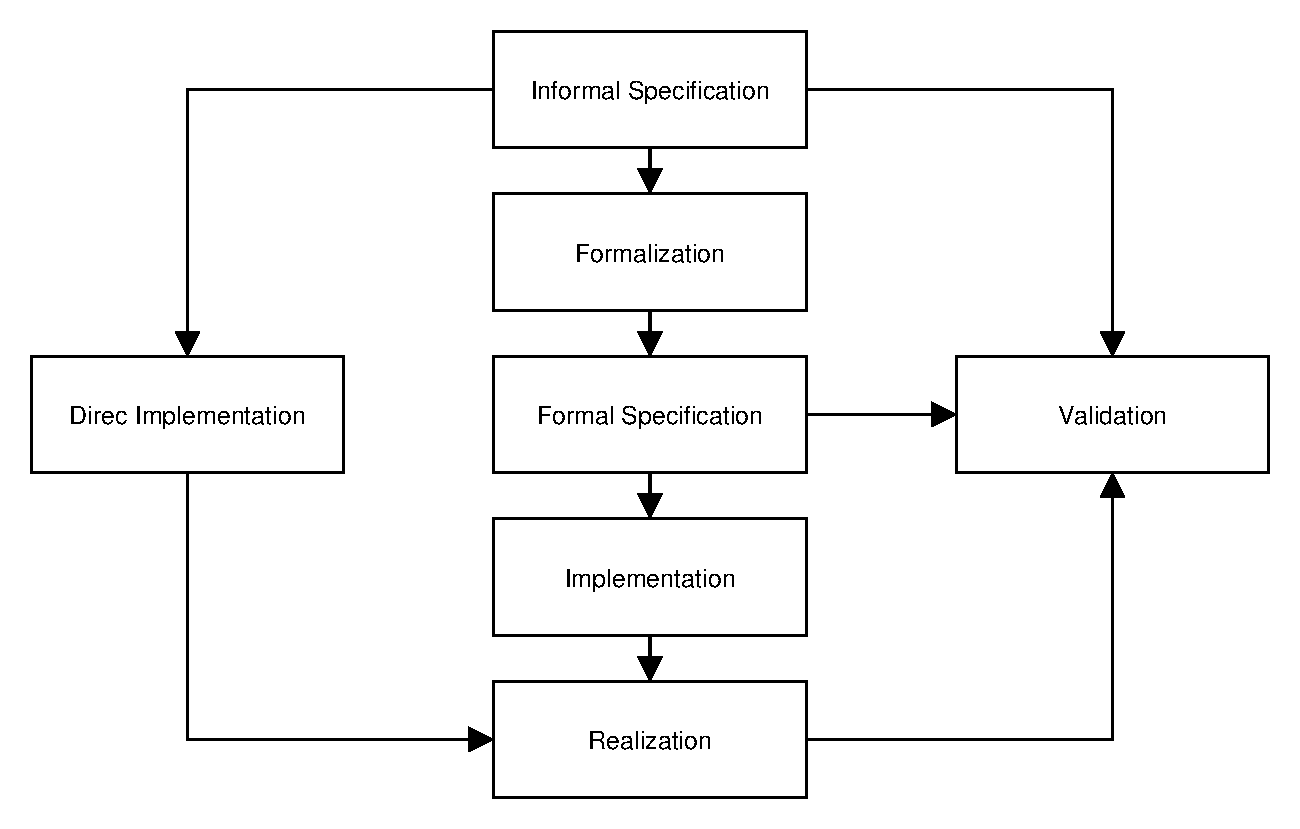
\includegraphics[width=\textwidth, keepaspectratio, angle=0]
  {forma_methods_in_design.pdf}
  \caption{Design process of automated systems}
  \label{fig:forma_methods_in_design}
\end{figure}

The Figure \ref{fig:forma_methods_in_design} depicts a generic model of a
manufacturing system design process. The design process of a particular system
starts, in most of the cases, with informal description of technological
processes. It specifies the system's behaviour in not a strictly semantically
and syntactically defined form. Additionally to the verbal form, the description
includes P\&I diagrams, equations and algorithms expressed in block diagrams.
The main problem with informal specifications is that they do not facilitate
tests for completeness, unambiguity and consistency of the system.

Until nowadays, the common approach is when after the stage of informal
specification immediately begins its direct implementation into a
code for {PLC} with a programming language. Instead, when applying formal
methods, the implementation stage follows after formalization of informal
descriptions into formal specification. Formalisation is performed by
humans, and involves conversion of textual and graphical information into the
form of a formal language or another representation (for instance, automata).

Formal specifications can be translated directly into programming languages
\cite{maclay_click_2000} by a design tool. This step eliminates the error prone
interpretation by humans ensuring that the system will behave exactly as it
was specified.

Formal specification of the system brings opportunity to apply 
\emph{verification} techniques to the design process. Verification is used
to prove some properties of the system's specification. These properties are
independent from the modeled system, such as, for example, existence of
deadlocks in the discrete-event systems approach.
Verification is closely related to \emph{Model checking} ``technique for
verifying finite state concurrent systems such as sequential circuit designs and
communication protocols. It has a number of advantages over traditional
approaches that are based on simulation, testing, and deductive
reasoning''\cite{clarke_model_1999}. Model checking verification considers a
system as state-based model specified using, for instance, automata framework,
and specifications of properties written in temporal logic.

A formal verification approach can be a model based or non model based. In 
model based approaches a model of the studied object is included into analysis.
This can be a model of technological process or of manufacturing equipment. In
non model based approaches the formal representation of specifications does not
include a model of the object. These approaches assume that, literally,
everything can happen. An example of this approach is development of a system
with a few formally described controllers, where the whole system, i.e. the
composition of the concurrent acting controllers needs to be verified for
deadlocks absence.

Due to importance of the problem of failures analysis for modern complex
automated systems, formal method tools are widely used to support it.
Whenever the specification of a system is accessible in a formal form, many
formal approaches can be applied for offline failure analyses of the system's
design and its online failures monitoring during its operation. 

The next Chapter \ref{chap:framework} describes an UML model based 
modeling approach for manufacturing systems design, and how this approach is
used to reflect failures, such that it is suitable for formal analysis due to
exploiting the automata framework at the internal layer. Then the
mathematical notation for discrete event systems is briefly presented,
different definitions of diagnosability are given, as well as an idea
underlining a new notion of diagnosability which is described in details in the
following Chapter \ref{chap:theory}.
